%% This is an example first chapter.  You should put chapter/appendix that you
%% write into a separate file, and add a line \include{yourfilename} to
%% main.tex, where `yourfilename.tex' is the name of the chapter/appendix file.
%% You can process specific files by typing their names in at the 
%% \files=
%% prompt when you run the file main.tex through LaTeX.
\chapter{Hardware Experiments}

\section{Centralized (WiFi) vs. Decentralized (Mesh) Network}

We tested RMADER on both centralized and decentralized communication networks. In a centralized network, a central machine, such as a WiFi router, handles all communication traffic. Note that the RMADER algorithm still runs onboard in a decentralized manner, even if the communication is centralized. On the other hand, in a decentralized (mesh) network, agents communicate directly with each other. 

Fig.~\ref{fig:network} illustrates a centralized and decentralized network. Although a centralized network is common in robotics, this approach could be subject to the failure of the central router and not be scalable.

Fig.~\ref{fig:comm_delay_on_mesh_centr} shows actual communication delays recorded on Exp. 1 - 23. Mesh network generally has smaller communication delays compared to WiFi; however, Mesh has a small number of large delays. 

\subsection{RMADER vs. MADER on Centralized (WiFi) Network}
 A total of 10 hardware experiments (5 flights for each) demonstrate RMADER's robustness to communication delays as well as MADER's shortcomings. Each flight test had 6 UAVs and lasted \SI{1}{\minute}. 

During the MADER hardware experiments, due to the effects of communication delays, \textbf{7} potential collisions were detected by the safety mechanism. RMADER, on the other hand, did not generate conflicts. 
A snapshot of one of the RMADER experiments is shown in Fig.~\ref{fig:rmader_centr}, and a successful trajectory deconfliction.
The maximum velocities and travel distances achieved during the hardware experiments are shown in Table~\ref{tab:mader_hw_centralized} and \ref{tab:rmader_hw_centralized}. Corresponding to simulation results in Section~\ref{sec:sim}, RMADER trades off safety with performance \textemdash Although MADER performs better than RMADER in average travel distance and stop time, RMADER did not show any collisions in these experiments. Note that we regarded a vehicle is stopped when its speed is less than \SI{0.1}{\m/\s}, and measured how long a vehicle was not moving in the experiment.

\subsection{RMADER on Decentralized (Mesh) Network}
We also performed RMADER on a mesh (decentralized) network, where the collision-safety boundary box around each UAV was set to \qtyproduct{0.8 x 0.8 x 1.0}{\m}, and the dynamic limits were set to \SI{2.0}{\m/\s}, \SI{3.0}{\m/\s^2}, and \SI{4.0}{\m/\s^3}, except for Experiment 5, where we relaxed the dynamic constraints to \SI{4.0}{\m/\s}, \SI{5.0}{\m/\s^2}, and \SI{6.0}{\m/\s^3}. Note that these dynamic constraints are element-wise - e.g., a UAV can achieve velocity up to $4\sqrt{3} \approx \SI{6.93}{m/s}$.

We observed a deadlock at the very end of Experiment 12. Compared to flight space, the boundary box used in these experiments is relatively large, and because we use hard constraints in trajectory optimization, this could occasionally lead to deadlock. Table~\ref{tab:rmader_hw_mesh} shows RMADER's performance on a mesh network, and Fig.~\ref{fig:6agent_mesh} illustrates 6 agents successfully carrying out deconfliction.

\begin{figure}[!htbp]
    \centering
    \begin{tikzpicture}
    \node (img) {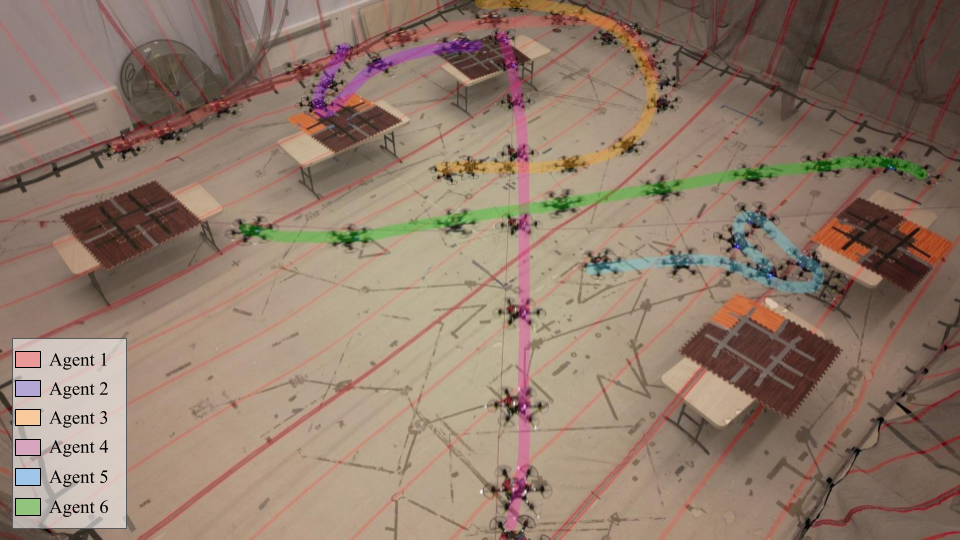
\includegraphics[width=\columnwidth, height=0.22\textheight, keepaspectratio]{figures/6agent_mesh.png}};
    %% circles
    \filldraw[color=black, fill=agent1_color] (-3.2, 1.1) circle (2pt);
    \filldraw[color=black, fill=agent2_color] (-1.2, 2) circle (2pt);
    \filldraw[color=black, fill=agent3_color] (0.05, 2.35) circle (2pt);
    \filldraw[color=black, fill=agent4_color] (0.3, -2.3) circle (2pt);
    \filldraw[color=black, fill=agent5_color] (2.6, 0) circle (2pt);
    \filldraw[color=black, fill=agent6_color] (4, 0.9) circle (2pt);
    %% squares
    \node [rectangle, draw, fill=agent1_color, inner sep=0.7mm] at (1.5, 1.8) {};
    \node [rectangle, draw, fill=agent2_color, inner sep=0.7mm] at (0, 2) {};
    \node [rectangle, draw, fill=agent3_color, inner sep=0.7mm] at (-0.3, 0.85) {};
    \node [rectangle, draw, fill=agent4_color, inner sep=0.7mm] at (0.2, 2.2) {};
    \node [rectangle, draw, fill=agent5_color, inner sep=0.7mm] at (1.1, 0) {};
    \node [rectangle, draw, fill=agent6_color, inner sep=0.7mm] at (-2.1, 0.35) {};
    \end{tikzpicture} 
    % \setlength{\belowcaptionskip}{-1em}
    \caption{\centering 6 agents on mesh network: Agents move from $\bigcircle$ to \protect\tikz \protect\node [rectangle,draw] at (0,0) {};. Snapshots shown every \SI{500}{ms}}
    \label{fig:6agent_mesh}
\end{figure}

\begin{table}
\caption{\centering RMADER on Mesh Metwork}
\label{tab:rmader_hw_mesh}
\begin{centering}
% test 2, 17, 19, 24, 30
\renewcommand{\arraystretch}{1.2}
\resizebox{1.0\columnwidth}{!}{
\begin{tabular}{ c c c c c c }
\toprule
 & \textbf{Exp. 11} & \textbf{Exp. 12} & \textbf{Exp. 13} & \textbf{Exp. 14} & \makecell{\textbf{Exp. 15} \\ (fast)}\tabularnewline
\hline 
\hline 
\textbf{Max vel. [m/s]} & 2.7 & 3.0 & 2.9 & 2.8 & 3.0\tabularnewline
\hline 
\textbf{Avg. travel distance [m]} & 46.9 & 48.0 & 49.4 & 66.6 & 60.3 \tabularnewline
\hline
\textbf{Stop time [s]} & 13.7 & 10.6 & 21.4 & 6.2 & 8.8 \tabularnewline
\bottomrule
\end{tabular}}
\par\end{centering}
\end{table}

\subsection{RMADER with Dynamic Obstacles on Mesh Network}
% 4agent2obs/test4, 7
% 6agent2obs/test10, 3, 11
This section illustrates a total of 8 hardware experiments (2 flights for 2 agents with a dynamic obstacle, 2 flights for 4 agents with 2 dynamic obstacles, and 3 flights for 6 agents with 2 dynamic obstacles). 2 and 4-agent experiments lasted \SI{1}{\minute}, and 6 agents exchange their position once. The dynamic constraints are \SI{3.0}{m/s}, \SI{4.0}{m/s^2}, and \SI{5.0}{m/s^3}, but in Experiments 20 and 23, we increased it up to \SI{5.0}{m/s}, \SI{7.0}{m/s^2}, and \SI{10.0}{m/s^3}, and the dynamic obstacles follow randomized trefoil trajectories. 
Table~\ref{tab:rmader_with_obstacles} shows RMADER's performance with obstacles, and Figs~\ref{fig:2agent1obs}, \ref{fig:4agent2obs}, and \ref{fig:6agent2obs} illustrate 2, 4, and 6 agents with RMADER running onboard successfully carrying out position exchange while avoiding dynamic obstacles.    
Note that due to a hardware issue, one of the 6 agents in Exp. 21-23 was not able to publish its trajectory; however, because it was receiving trajectories from other agents and because of RMADER's decentralized deconfliction mechanism, we observed no collisions. 

\begin{table}
\caption{\centering Hardware experiments with dynamic obstacles}
\label{tab:rmader_with_obstacles}
\begin{centering}
\renewcommand{\arraystretch}{1.2}
\resizebox{1.0\columnwidth}{!}{
\begin{tabular}{ c c c | c c c | c c c }
\toprule
& \multicolumn{2}{c}{\makecell{\textbf{2 agents} \\ (1min)}} & \multicolumn{3}{c}{\makecell{\textbf{4 agents} \\ (1min) }} &  \multicolumn{3}{c}{\makecell{\textbf{6 agents} \\ (one time) }}\tabularnewline
 & \textbf{Exp. 16} & \textbf{Exp. 17} & \textbf{Exp. 18} & \textbf{Exp. 19} & \makecell{\textbf{Exp. 20} \\ (fast)} & \textbf{Exp. 21} & \textbf{Exp. 22} & \makecell{\textbf{Exp. 23} \\ (fast)}  \tabularnewline
\hline 
\hline 
\textbf{Max vel. [m/s]} & 2.9 & 2.9 & 3.8 & 3.6 & 5.8 & 3.2 & 3.5 & 5.6 \tabularnewline
\hline 
\makecell{\textbf{Avg. travel} \\ \textbf{distance [m]}} & 117.5 & 120.6 & 114.9 & 109.9 & 114.4 & 24.6 & 23.7 & 22.2 \tabularnewline
\hline
\textbf{Stop time [s]} & 0.30 & 0.91 & 3.51 & 0.90 & 4.91 & 2.42 & 0.76 & 0.76 \tabularnewline
\bottomrule
\end{tabular}
}
\par\end{centering}
\end{table}

\begin{figure}[!htbp]
    \centering
    \begin{tikzpicture}
    \node (img) {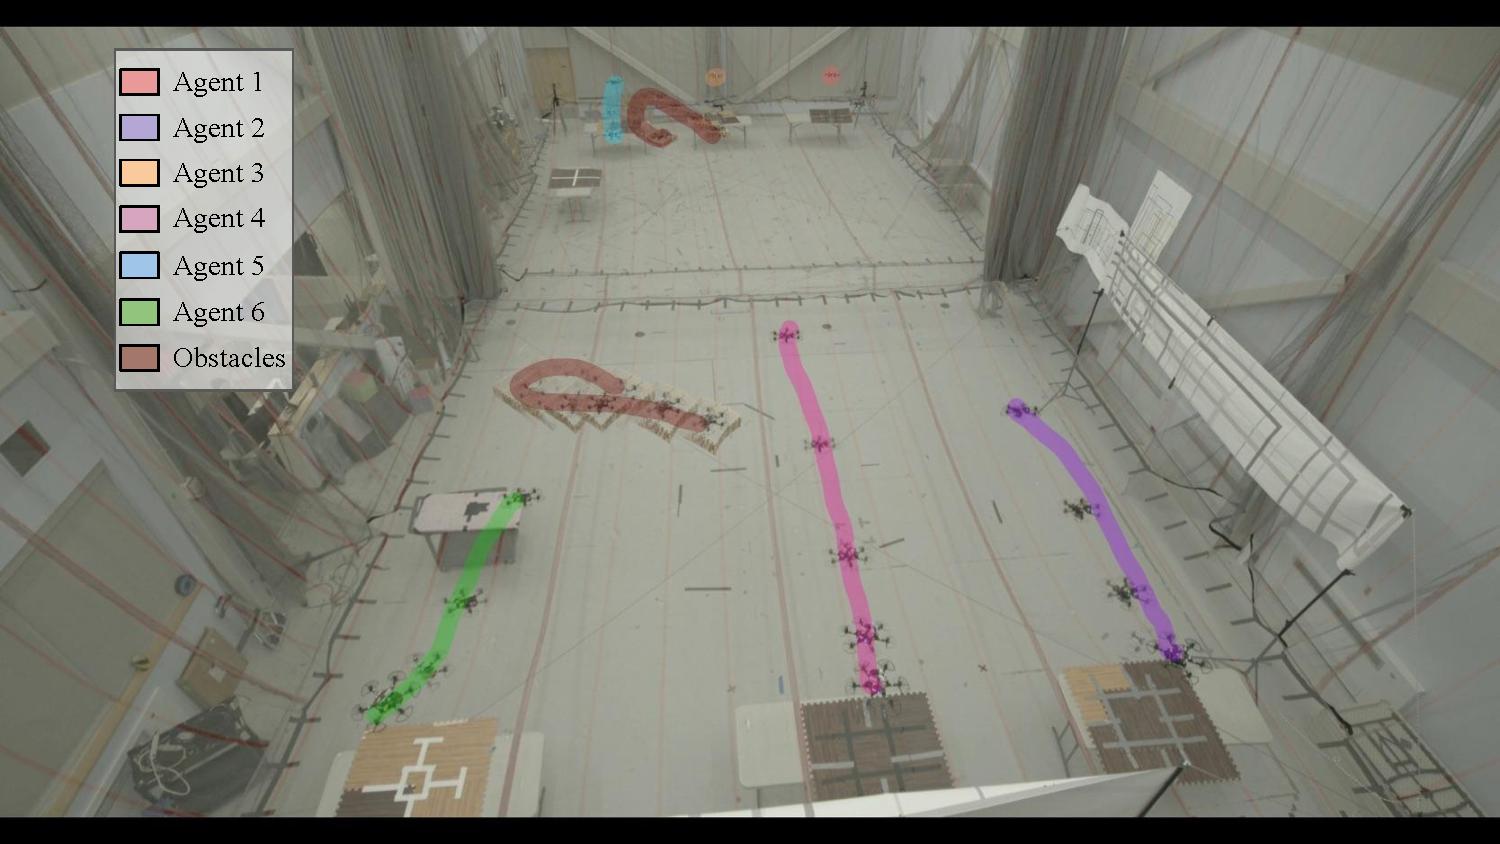
\includegraphics[width=\columnwidth, height=0.22\textheight, trim={1.8cm 1cm 3cm 0.7cm}, clip, keepaspectratio]{figures/rmader_hw_six_agents1_legend.pdf}};
    \node [rectangle, draw, fill=agent1_color, inner sep=0.5mm] at (1.2, 2.45) {\tiny start};
    \node [rectangle, draw, fill=agent2_color, inner sep=0.5mm] at (3, -2) {\tiny start};
    \node [rectangle, draw, fill=agent3_color, inner sep=0.5mm] at (0.4, 2.45) {\tiny start};
    \node [rectangle, draw, fill=agent4_color, inner sep=0.5mm] at (1.3, -2.1) {\tiny start};
    \node [rectangle, draw, fill=agent5_color, inner sep=0.5mm] at (-0.5, 2.45) {\tiny start};
    \node [rectangle, draw, fill=agent6_color, inner sep=0.5mm] at (-2, -2.3) {\tiny start};
    \filldraw[color=black, fill=agent1_color] (0.8, 2.4) circle (2pt);
    \filldraw[color=black, fill=agent2_color] (2.1, 0) circle (2pt);
    \filldraw[color=black, fill=agent3_color] (0, 2.4) circle (2pt);
    \filldraw[color=black, fill=agent4_color] (0.5, 0.5) circle (2pt);
    \filldraw[color=black, fill=agent5_color] (-0.7, 1.9) circle (2pt);
    \filldraw[color=black, fill=agent6_color] (-1.3, -0.5) circle (2pt);
    \end{tikzpicture} 
    {\scriptsize $t=$ \SIrange{0}{5}{\s}: Agents move from \mybox[fill=white, draw]{start} to $\bigcircle$}
    \begin{tikzpicture}
    \node (img) {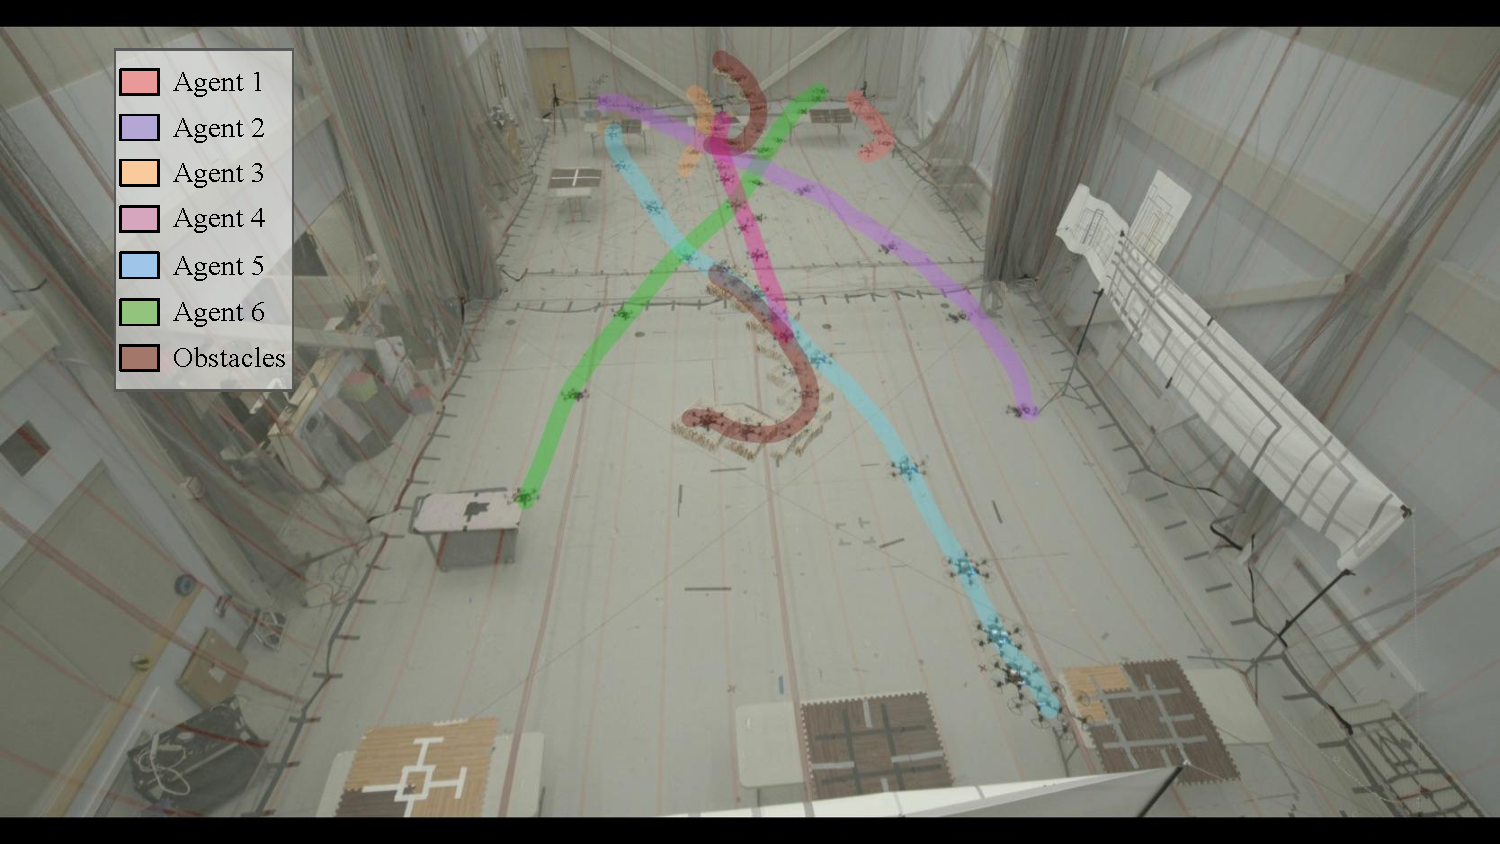
\includegraphics[width=\columnwidth, height=0.22\textheight, trim={1.8cm 1cm 3cm 0.7cm}, clip, keepaspectratio]{figures/rmader_hw_six_agents2_legend.pdf}};
    %% circles
    \filldraw[color=black, fill=agent1_color] (1.0, 2.2) circle (2pt);
    \filldraw[color=black, fill=agent2_color] (2.2, 0) circle (2pt);
    \filldraw[color=black, fill=agent3_color] (-0.1, 2.3) circle (2pt);
    \filldraw[color=black, fill=agent4_color] (0.5, 0.5) circle (2pt);
    \filldraw[color=black, fill=agent5_color] (-0.7, 1.9) circle (2pt);
    \filldraw[color=black, fill=agent6_color] (-1.3, -0.5) circle (2pt);
    %% squares
    \node [rectangle, draw, fill=agent1_color, inner sep=0.7mm] at (1.1, 1.8) {};
    \node [rectangle, draw, fill=agent2_color, inner sep=0.7mm] at (-0.8, 2.3) {};
    \node [rectangle, draw, fill=agent3_color, inner sep=0.7mm] at (-0.2, 1.7) {};
    \node [rectangle, draw, fill=agent4_color, inner sep=0.7mm] at (0.1, 2.2) {};
    \node [rectangle, draw, fill=agent5_color, inner sep=0.7mm] at (2.4, -2.2) {};
    \node [rectangle, draw, fill=agent6_color, inner sep=0.7mm] at (0.8, 2.3) {};
    \end{tikzpicture}
    {\scriptsize $t=$ \SIrange{5}{10}{\s}: Agents move from $\bigcircle$ to \ \rectangle}
    \begin{tikzpicture}
    \node (img) {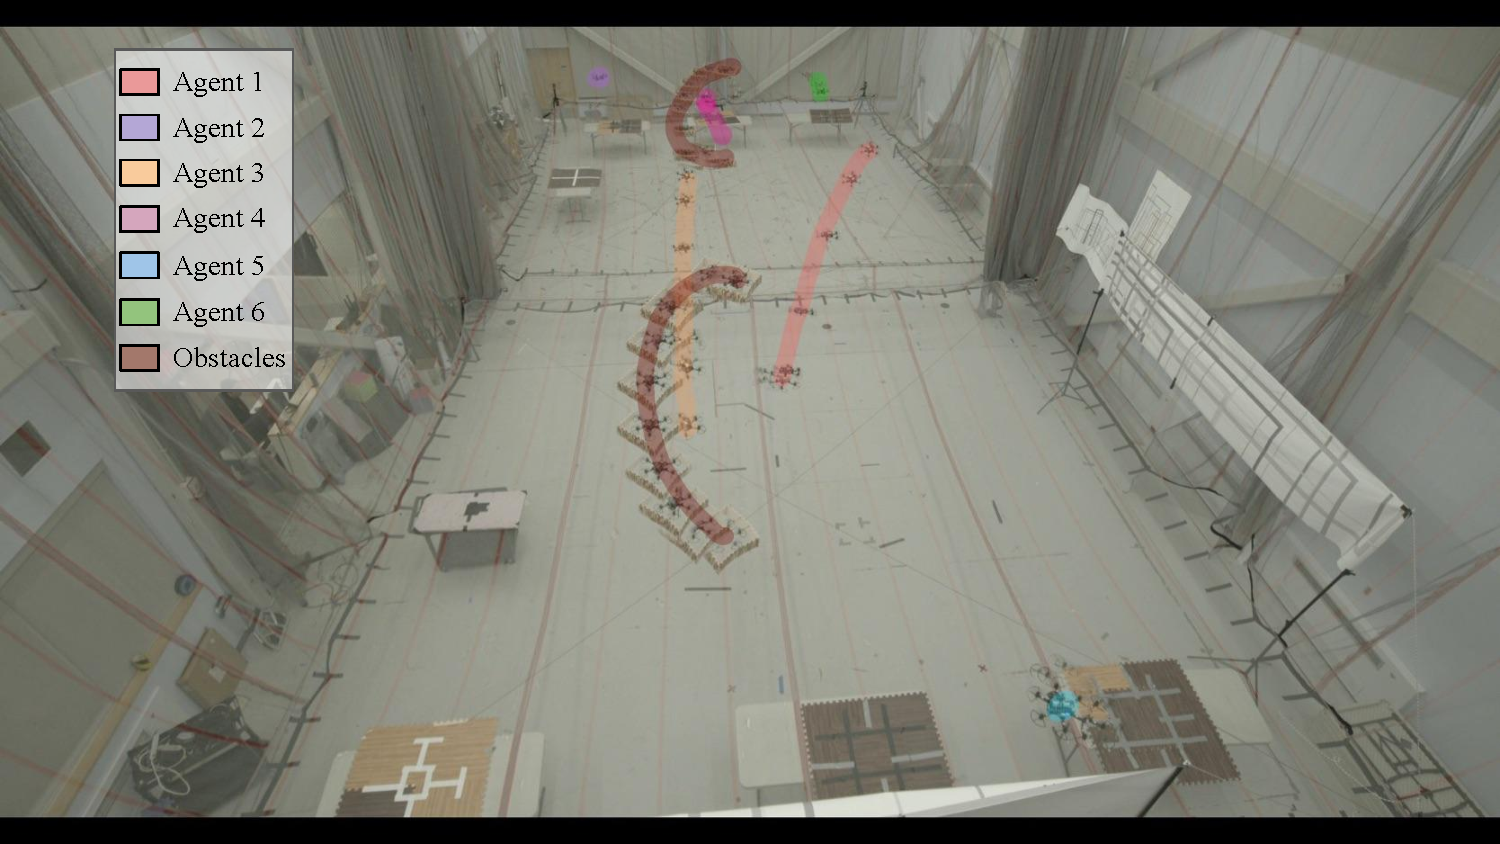
\includegraphics[width=\columnwidth, height=0.22\textheight, trim={1.8cm 1cm 3cm 0.7cm}, clip, keepaspectratio]{figures/rmader_hw_six_agents3_legend.pdf}};
    %% rectangle
    \node [rectangle, draw, fill=agent1_color, inner sep=0.7mm] at (1.2, 1.9) {};
    \node [rectangle, draw, fill=agent3_color, inner sep=0.7mm] at (-0.2, 1.6) {};
    \node [rectangle, draw, fill=agent4_color, inner sep=0.7mm] at (0.1, 1.9) {};
    %% triangle
    \node [regular polygon, regular polygon sides=3, draw, fill=agent1_color, inner sep=0.4mm] at (0.5, 0.2) {};
    % \node [regular polygon, regular polygon sides=3, draw, fill=agent2_color, inner sep=0.4mm] at (0.5, 0.2) {};
    \node [regular polygon, regular polygon sides=3, draw, fill=agent3_color, inner sep=0.4mm] at (-0.1, -0.2) {};
    \node [regular polygon, regular polygon sides=3, draw, fill=agent4_color, inner sep=0.4mm] at (-0.1, 2.2) {};
    % \node [regular polygon, regular polygon sides=3, draw, fill=agent5_color, inner sep=0.4mm] at (0.5, 0.2) {};
    % \node [regular polygon, regular polygon sides=3, draw, fill=agent6_color, inner sep=0.4mm] at (0.5, 0.2) {};
    %% goal
    \node [rectangle, draw, fill=agent2_color, inner sep=0.5mm] at (-1.0, 2.3) {\tiny goal};
    \node [rectangle, draw, fill=agent5_color, inner sep=0.5mm] at (2.5, -2.2) {\tiny goal};
    \node [rectangle, draw, fill=agent6_color, inner sep=0.5mm] at (1.0, 2.3) {\tiny goal};
    \end{tikzpicture}
    {\scriptsize $t=$ \SIrange{10}{15}{\s}: Agents move from \rectangle \ to $\triangle$. Agents 2, 5, and 6 reached the goal.}
    \begin{tikzpicture}
    \node (img) {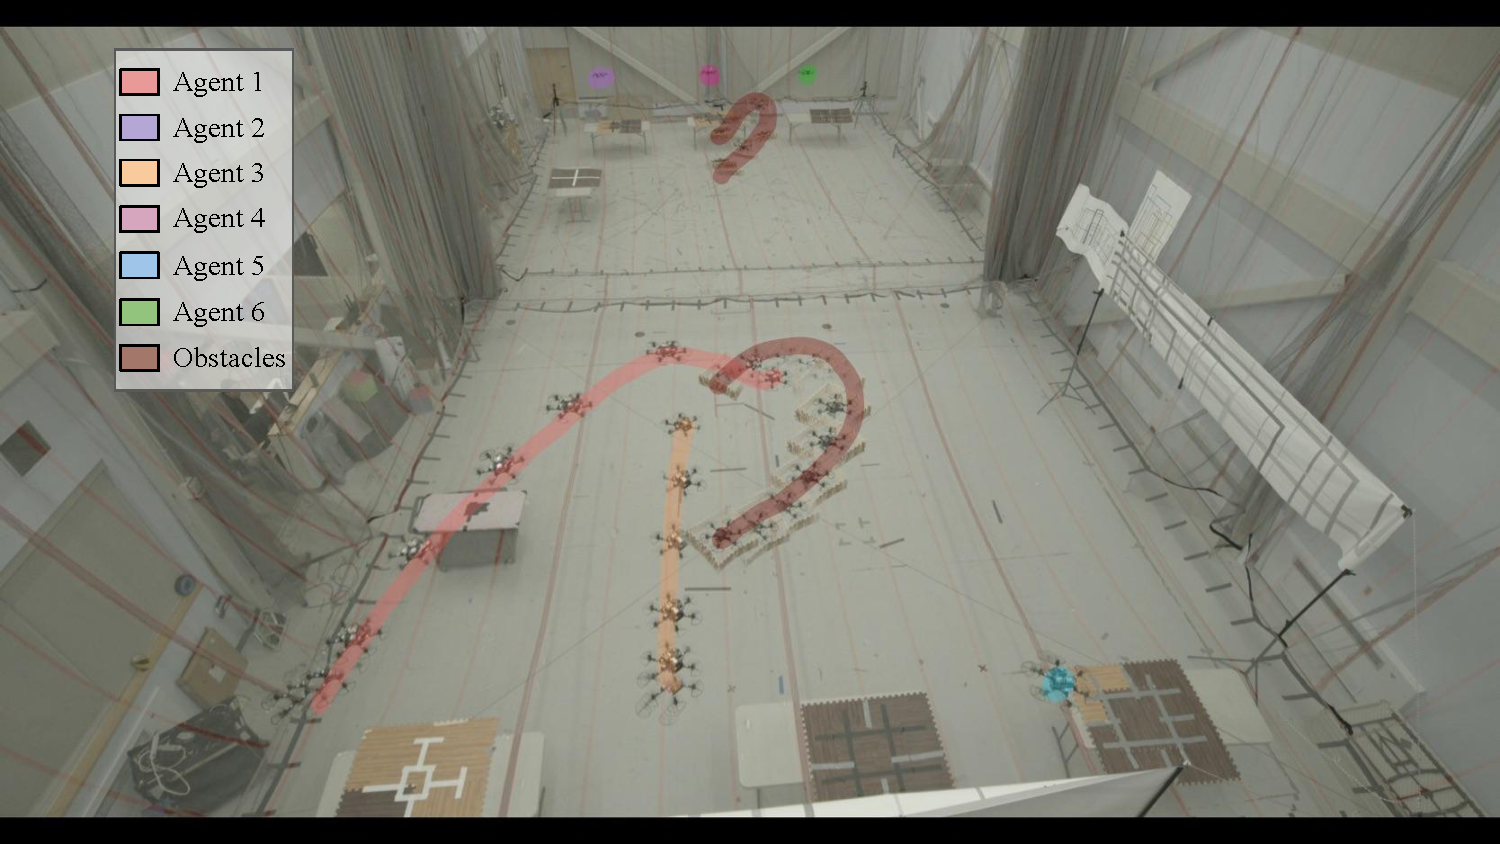
\includegraphics[width=\columnwidth, height=0.22\textheight, trim={1.8cm 1cm 3cm 0.7cm}, clip, keepaspectratio]{figures/rmader_hw_six_agents4_legend.pdf}};
    \node [regular polygon, regular polygon sides=3, draw, fill=agent1_color, inner sep=0.4mm] at (0.5, 0.2) {};
    \node [regular polygon, regular polygon sides=3, draw, fill=agent3_color, inner sep=0.4mm] at (-0.1, -0.2) {};
    %% goal
    \node [rectangle, draw, fill=agent1_color, inner sep=0.5mm] at (-2.7, -2.1) {\tiny goal};
    \node [rectangle, draw, fill=agent2_color, inner sep=0.5mm] at (-1.0, 2.3) {\tiny goal};
    \node [rectangle, draw, fill=agent3_color, inner sep=0.5mm] at (-0.2, -2.1) {\tiny goal};
    \node [rectangle, draw, fill=agent4_color, inner sep=0.5mm] at (0.3, 2.3) {\tiny goal};
    \node [rectangle, draw, fill=agent5_color, inner sep=0.5mm] at (2.5, -2.2) {\tiny goal};
    \node [rectangle, draw, fill=agent6_color, inner sep=0.5mm] at (1.0, 2.3) {\tiny goal};
    \end{tikzpicture}
    {\scriptsize $t=$ \SIrange{15}{20}{\s}: Agents move from $\triangle$ to \mybox[fill=white, draw]{goal} }
    \setlength{\belowcaptionskip}{-1em}
    \caption{\centering 6 agent hardware experiments with 2 dynamic obstacles. Snapshots shown every \SI{500}{ms}}
    \label{fig:rmader_6_agents_with_2_dyn_obs}
\end{figure}

\begin{figure}[!htbp]
    \centering
    \begin{tikzpicture}
    \node (img) {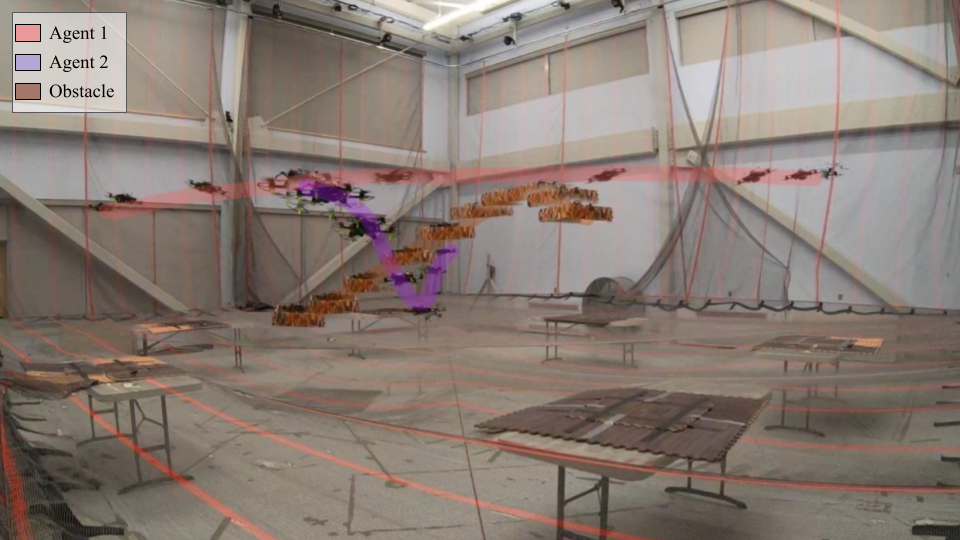
\includegraphics[width=\columnwidth, height=0.22\textheight, clip, keepaspectratio]{figures/2agent1obs.png}};
    %% circles
    \filldraw[color=black, fill=agent1_color] (3.1, 0.85) circle (2pt);
    \filldraw[color=black, fill=agent2_color] (-1.4, 0.7) circle (2pt);
    \filldraw[color=black, fill=obstacle_color] (0.9, 0.5) circle (2pt);
    %% squares
    \node [rectangle, draw, fill=agent1_color, inner sep=0.7mm] at (-3.3, 0.6) {};
    \node [rectangle, draw, fill=agent2_color, inner sep=0.7mm] at (-0.4, 0.2) {};
    \node [rectangle, draw, fill=obstacle_color, inner sep=0.7mm] at (-1.6, -0.4) {};

    \end{tikzpicture} 
    % \setlength{\belowcaptionskip}{-1em}
    \caption{\centering 2 agents with a dynamic obstacle: agents move from $\bigcircle$ to \protect\tikz \protect\node [rectangle,draw] at (0,0) {};. Snapshots shown every \SI{500}{ms}}
    \label{fig:2agent1obs}
\end{figure}

\begin{figure}[!htbp]
    \centering
    \begin{tikzpicture}
    \node (img) {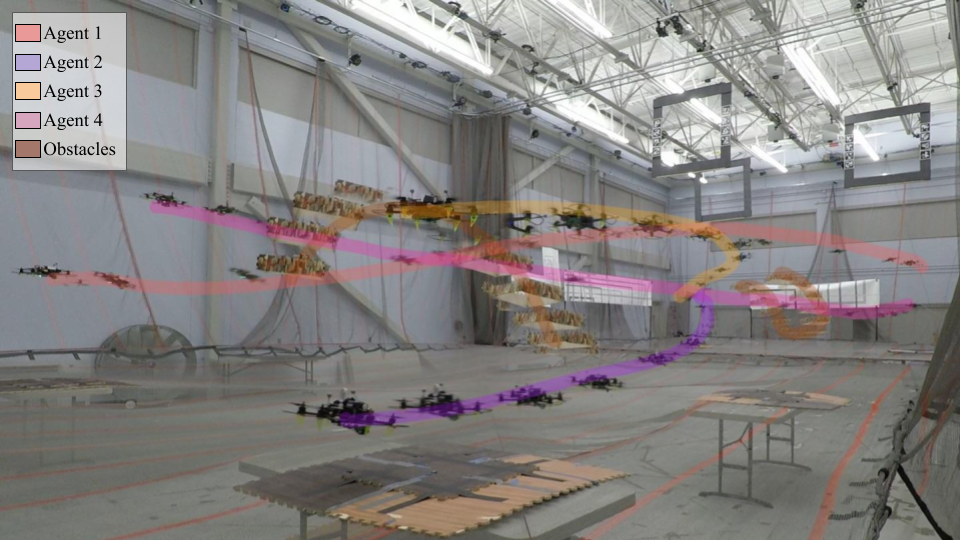
\includegraphics[width=\columnwidth, height=0.22\textheight, keepaspectratio]{figures/4agent2obs.png}};
    %% circles
    \filldraw[color=black, fill=agent1_color] (-3.9, -0.1) circle (2pt);
    \filldraw[color=black, fill=agent2_color] (1.9, -0.2) circle (2pt);
    \filldraw[color=black, fill=agent3_color] (-0.7, 0.5) circle (2pt);
    \filldraw[color=black, fill=agent4_color] (3.8, -0.3) circle (2pt);
    \filldraw[color=black, fill=obstacle_color] (-1.65, 0.05) circle (2pt);
    \filldraw[color=black, fill=obstacle_color] (2.6, 0) circle (2pt);
    %% squares
    \node [rectangle, draw, fill=agent1_color, inner sep=0.7mm] at (3.9, 0) {};
    \node [rectangle, draw, fill=agent2_color, inner sep=0.7mm] at (-1.1, -1.4) {};
    \node [rectangle, draw, fill=agent3_color, inner sep=0.7mm] at (1.8, -0.2) {};
    \node [rectangle, draw, fill=agent4_color, inner sep=0.7mm] at (-2.8, 0.6) {};
    \node [rectangle, draw, fill=obstacle_color, inner sep=0.7mm] at (0.65, -0.7) {};
    \node [rectangle, draw, fill=obstacle_color, inner sep=0.7mm] at (2.35, -0.2) {};
    
    \end{tikzpicture} 
    % \setlength{\belowcaptionskip}{-1em}
    \caption{\centering 4 agents with 2 dynamic obstacles: agents move from $\bigcircle$ to \protect\tikz \protect\node [rectangle,draw] at (0,0) {};. Snapshots shown every \SI{500}{ms}}
    \label{fig:4agent2obs}
\end{figure}

\begin{figure}[!htbp]
    \centering
    \begin{tikzpicture}
    \node (img) {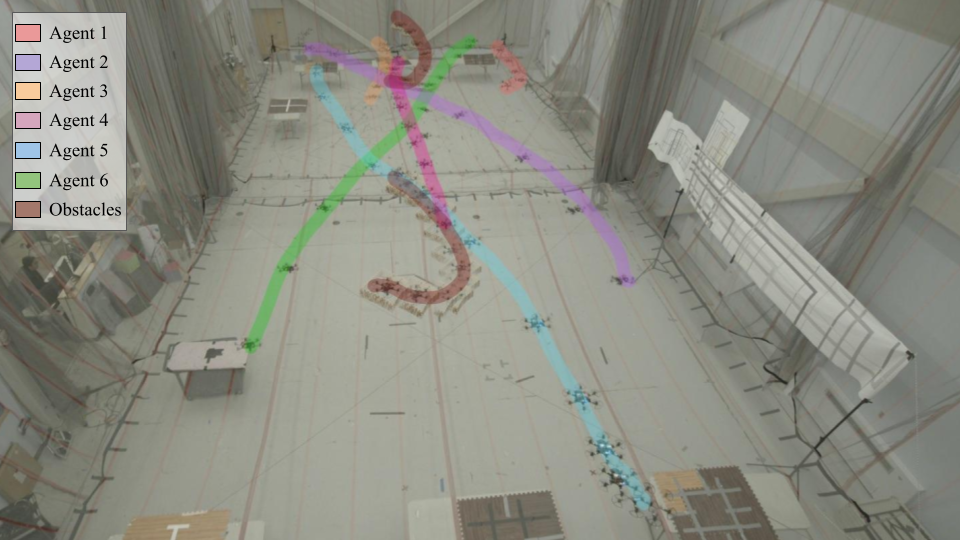
\includegraphics[width=\columnwidth, height=0.22\textheight, keepaspectratio]{figures/6agent2obs.png}};
    %% circles
    \filldraw[color=black, fill=agent1_color] (0.2, 2.0) circle (2pt);
    \filldraw[color=black, fill=agent2_color] (1.3, -0.05) circle (2pt);
    \filldraw[color=black, fill=agent3_color] (-0.9, 2) circle (2pt);
    \filldraw[color=black, fill=agent4_color] (-0.3, 0.5) circle (2pt);
    \filldraw[color=black, fill=agent5_color] (-1.5, 1.9) circle (2pt);
    \filldraw[color=black, fill=agent6_color] (-2.0, -0.7) circle (2pt);
    \filldraw[color=black, fill=obstacle_color] (-0.9, -0.15) circle (2pt);
    \filldraw[color=black, fill=obstacle_color] (-0.7, 1.7) circle (2pt);
    %% squares
    \node [rectangle, draw, fill=agent1_color, inner sep=0.7mm] at (0.2, 1.6) {};
    \node [rectangle, draw, fill=agent2_color, inner sep=0.7mm] at (-1.6, 2) {};
    \node [rectangle, draw, fill=agent3_color, inner sep=0.7mm] at (-1, 1.4) {};
    \node [rectangle, draw, fill=agent4_color, inner sep=0.7mm] at (-0.8, 1.8) {};
    \node [rectangle, draw, fill=agent5_color, inner sep=0.7mm] at (1.6, -2.2) {};
    \node [rectangle, draw, fill=agent6_color, inner sep=0.7mm] at (0, 2.1) {};
    \node [rectangle, draw, fill=obstacle_color, inner sep=0.7mm] at (-0.7, 2.3) {};
    \node [rectangle, draw, fill=obstacle_color, inner sep=0.7mm] at (-0.8, 0.8) {};
    \end{tikzpicture}
    \caption{6 agents with 2 dynamic obstacles: agents move from $\bigcircle$ to \protect\tikz \protect\node [rectangle,draw] at (0,0) {};}
    \label{fig:6agent2obs}
\end{figure}